\section{Motivation}\label{sec:motivation}

Contemporary optimizing compilers are mainly based on variants of the control flow
graph as imperative program representations. %
These representations preserve sequential execution semantics of the input program, such as access order of aliased references.
The LLVM representation is based on the instruction set
of a virtual CPU with operation semantics resembling real CPUs. %
This choice of representation is somewhat at odds with the requirements of code
optimization analysis, which often focuses on {\em data dependence} instead.
As Table~\ref{tab:llvm-opts} shows, most executed optimization passes
are concerned with data flow analysis in the form of SSA construction
and interpretation, or in-memory data structures in the form of alias analysis
and/or memory SSA. %

We propose the data-dependence centric RVSDG as an alternative. %
While it requires more effort to construct the RVSDG from imperative
programs and recover control flows for code generation, we believe this cost
is more than recovered by benefits to analyses and optimizations.
The following sections provide illustrative examples.

\begin{wraptable}{l}{0.5\textwidth}
  \vspace{-1em}
	\caption{Thirteen most invoked LLVM 7.0.1 passes at \texttt{O3}.\label{tab:llvm-opts}}
	\resizebox{0.5\textwidth}{!}{%
	\begin{tabular}{l|c}
		Optimization                                                             & \# Invocations\\\hline\hline
		1. Alias Analysis (\texttt{-aa})                                         & 19\\
		2. Basic Alias Analysis (\texttt{-basicaa})                              & 18\\
		3. Optimization Remark Emitter (\texttt{-opt-remark-emitter})            & 15\\
		4. \textbf{Natural Loop Information (\texttt{-loops})}                   & 14\\
		5. Lazy Branch Probability Analysis (\texttt{-lazy-branch-prob})         & 14\\
		6. Lazy Block Frequency Analysis (\texttt{-lazy-block-freq})             & 14\\
		7. \textbf{Dominator Tree Construction (\texttt{-domtree})}              & 13\\
		8. Scalar Evolution Analysis (\texttt{-scalar-evolution})                & 10\\
		9. \textbf{CFG Simplifier (\texttt{-simplifycfg})}                       & 8\\
		10. Redundant Instruction Combinator (\texttt{-instcombine})             & 8\\
		11. \textbf{Natural Loop Canonicalization (\texttt{-loop-simplify})}     & 8\\
		12. \textbf{Loop-Closed SSA Form (\texttt{-lcssa})}                      & 7\\
		13. \textbf{Loop-Closed SSA Form Verifier (\texttt{-lcssa-verification})}& 7\\\hline
		Total                                                                    & 155\\\hline
		\textbf{SSA Restoration}                                                 & 14\\
	\end{tabular}
      }
  \vspace{-1em}
\end{wraptable}

\begin{figure*}
	\subfloat[Code\label{fig:exp1-code}]{
		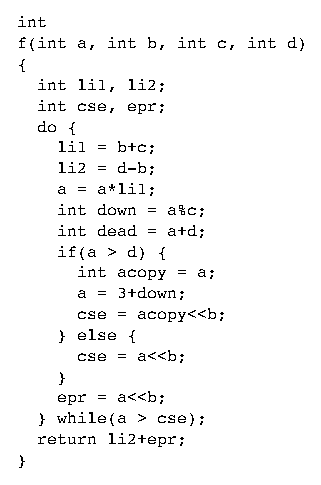
\includegraphics[scale=0.95]{example1}
	}
	\hfill
	\subfloat[CFG in SSA form\label{fig:exp1-cfg}]{
		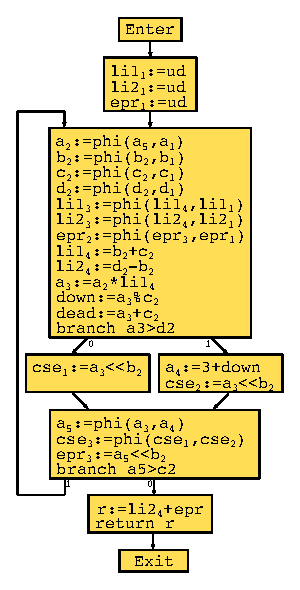
\includegraphics[scale=0.95]{example1_cfg}
	}
	\hfill
	\subfloat[Unoptimized RVSDG\label{fig:exp1-rvsdg}]{
		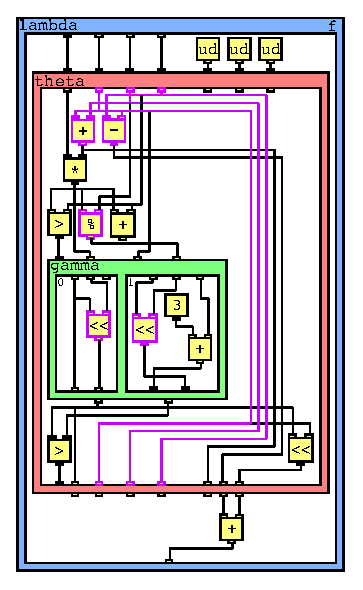
\includegraphics[scale=0.95]{example1_rvsdg}
	}

	\subfloat[Optimized RVSDG\label{fig:exp1-rvsdg-opt}]{
		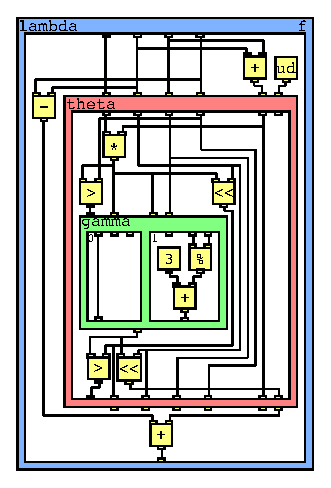
\includegraphics[scale=0.95]{example1_rvsdg-opt}
	}
	\hfill
	\subfloat[Code\label{fig:exp2-code}]{
		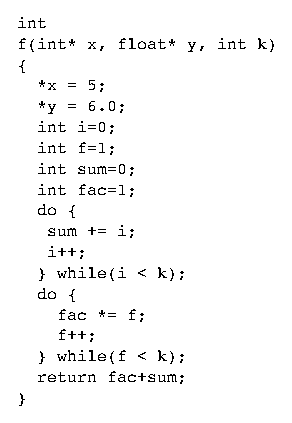
\includegraphics[scale=0.95]{example2}
	}
	\hfill
	\subfloat[RVSDG of Code~\ref{fig:exp2-code}\label{fig:exp2-rvsdg}]{
		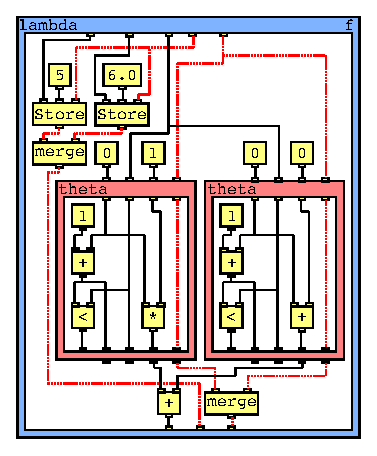
\includegraphics[scale=0.95]{example2-rvsdg}
	}
	\caption{RVSDG Examples}
	\label{fig:exp1}
\end{figure*}

\subsection{Simplified Compilation by Strong Representation Invariants}\label{sec:rep-invariants}

The Control Flow Graph (CFG) in Static Single Assignment (SSA)
form~\cite{Cytron91} is the dominant IR for optimizations in modern
imperative language compilers~\cite{Stanier13}. %
Its nodes represent a list of totally ordered operations, and its edges a
program's possible control flow paths, permitting efficient control flow
optimizations and simple code generation. %
The CFG's translation to SSA form improves the efficiency of many data flow
optimizations~\cite{Rosen88,Wegman91}. %
Figure~\ref{fig:exp1-code} shows a function with a simple loop and a
conditional, and Figure~\ref{fig:exp1-cfg} shows the
corresponding~CFG~in~SSA~form. %

SSA form is not an intrinsic property of the CFG, but a
specialized variant that must be actively maintained. %
Compiler passes such as jump threading or live-range splitting may perform
transformations that cause the CFG to no longer satisfy this form. %
As shown in Table~\ref{tab:llvm-opts}, LLVM requires SSA restoration~\cite{Choi96} in 14 different
passes.

Moreover, CFG-based compilers must frequently (re-)discover and canonicalize loops,
or establish various invariants besides SSA form. %
Table~\ref{tab:llvm-opts} shows that six of the 13 most invoked passes in LLVM
only perform such tasks, and account for 21\% of all invocations. %
This lack of invariants complicates implementation of optimizations
and analyses, increases engineering effort, prolongs compilation
time, and leads to compiler bugs~\cite{llvm-bug1,llvm-bug2,llvm-bug3}. %

In contrast, the RVSDG is always in strict SSA form as edges connect each operand
input to only one output. It explicitly exposes program structures such as loops
in a tree structure (Section~\ref{sec:rvsdg}), similarly to the Program Structure
Tree~\cite{Johnson94}. This makes SSA restoration and the other helper passes
from Table~\ref{tab:llvm-opts} redundant.
Figure \ref{fig:exp1-rvsdg} shows the RVSDG corresponding
to Figure \ref{fig:exp1-code}. %
It is an acyclic demand-dependence graph where nodes represent simple operations
or control flow constructs, and edges represent dependencies between
computations (Section~\ref{sec:rvsdg}). %
In Figure \ref{fig:exp1-rvsdg}, simple operations are colored yellow,
conditionals are green, loops are red, and functions are blue. %

\subsection{Unified Representation of Different Levels of Program Structures}

While the CFG can represent %
a single procedure, representation of programs as a whole requires additional
data structures such as call graphs. %
The RVSDG can represent a program as a unified data structure where a def-use
dependency of one function on another is modeled the same way as the def-use
dependency of scalar quantities. %
This makes it possible to apply the same transformation at multiple levels,
and considerably reduce the number of transformation passes and
algorithms, \eg, by uniform treatment of unreachable code, dead function analysis,
 and dead variable analysis (Section~\ref{sec:dne}).

\subsection{Strongly Normalized Representation}

The RVSDG program representation is much more strongly normalized than control flow
representations. %
Programs differing only in the ordering of (independent) operations result in
the same RVSDG representation, while state edges ensure the correct evaluation order
of stateful computations. Loops and conditionals always take a single
canonical form. %
These normalizations already simplify the implementation of
transformations~\cite{Weise94,Johnson04,Lawrence07} and eliminate the need for (repeated)
compiler analysis passes such as loop detection. %

Some common program optimizing transformations take a particular simple form in
the RVSDG representation. %
For example, Figure~\ref{fig:exp1-rvsdg-opt} shows the optimized RVSDG of
Figure~\ref{fig:exp1-rvsdg}, illustrating some of these optimizations: %
The inputs to the ``upper left'' plus operation are easily recognized as loop
invariant because their ``loop entry ports'' connect directly to the
corresponding ``loop exit ports'' (operations, ports, and edges highlighted in
purple). %
A simple push strategy allows to recursively identify data dependent operations
as invariant and hoist them out of the loop: %
The addition and subtraction computing \verb;li1; and \verb;li2; are moved out
of the loop (theta) as their operands, \ie, \verb;b;, \verb;c;, and \verb;d;, are
loop invariant (all three of them connect the entry of the loop to the exit). %
Similarly, the shift operation common to both conditional branches is hoisted
and combined, while the division operation is moved into the conditional as it
is only used in one alternative. %
In contrast to CFG-based compilers, all these optimizations are performed
directly on the unoptimized RVSDG of Figure~\ref{fig:exp1-rvsdg} and can be
performed in a single regular pass. %
No additional data structures or helper passes are required. %
See also Section~\ref{sec:optimizations} for further details. %

\subsection{Exposing Independent Computations}

CFGs implicitly represent a single global machine state by sequencing every 
operation that affects it. While RVSDG can model the same machine,
it is not limited to this interpretation. %
The RVSDG can also model systems consisting of multiple
{\em independent} states. Figures~\ref{fig:exp2-code},\ref{fig:exp2-rvsdg}
illustrate this concept with a function that contains two non-aliasing store
operations (targeting memory objects of incompatible types) and two
independent loops.

In a CFG, both stores and loops are strictly ordered. Their
mutual independence needs to be established by explicit compiler passes (and
may need to be re-established multiple times during the compilation
process as the number of alias analysis passes in Table~\ref{tab:llvm-opts} illustrate)
and represented using auxiliary data structures and/or annotations. In
contrast, the RVSDG permits the encoding of such information directly in the graph, as shown in
Figure~\ref{fig:exp2-rvsdg}. Disjoint memory regions (consisting of {\tt int}-typed
and {\tt float}-typed memory objects) are modeled as disjoint states, exposing
the independence of affecting operations in the representation. RVSDG can
in principle go even further in representing a {\em memory SSA} form that is
not formally any different from {\em value SSA} form, enabling the same kind
of optimizations to be applied to both.

\subsection{Multiple levels of abstraction}

The RVSDG is fairly abstract in nature and can contain operational nodes at vastly
different abstraction levels: Operational nodes may closely correspond to ``source
code'' level constructs operating on data structures modeled as state, or may
map to individual machine instructions affecting machine and memory state. This
offers an opportunity to structure compilers in a way that can preserve
considerably more source code semantics and utilize it at any later stage in the
translation. For example, contents of two distinct {\tt std::vector} instances
can never alias by language semantics, but this fact is entirely lost on
present-day compilers due to early lowering into a machine-like representation
without the capability to convey such high-level semantics. The RVSDG does not face
any such limitations (vector contents could be modeled as independent states
from the very beginning), can optimize at multiple levels of abstraction,
and can preserve vital invariants across abstraction levels. We expect this effect to become
particularly pronounced the more input programs are formulated above the abstraction level
of the C language, \eg, functional languages or languages expressing contracts
on affected state.


\subsection{Summary}

The RVSDG raises the IR abstraction level by enforcing desirable properties, such as
SSA form, explicitly encoding important structures, such as loops, and relaxing the overly strict
order of the input program. This leads to a more normalized program representation and avoids
many idiosyncrasies and artifacts from other IRs, such as the CFG, and further helps to expose
parallelism in programs.

